% Project report for nano-coder.
% Build:  pdflatex -interaction=nonstopmode report.tex   (twice, for refs)
% Figures come from report/make_figures.py, which reads runs/metrics/*.jsonl.
\documentclass[10pt,a4paper]{article}
\usepackage[margin=2.1cm]{geometry}
\usepackage{graphicx,booktabs,xcolor,amsmath,amssymb}
% expansion=false: pdfTeX refuses to auto-expand the non-scalable inconsolata
% bitmaps and dies outright rather than warning.
\usepackage[expansion=false]{microtype}
\usepackage{lmodern}
\usepackage[colorlinks=true,linkcolor=linknavy,urlcolor=linknavy,citecolor=linknavy]{hyperref}
\usepackage{titlesec,enumitem,caption,longtable,array,tcolorbox}
\usepackage{inconsolata}

\definecolor{ink}{HTML}{16324F}
\definecolor{acc}{HTML}{B3402F}
\definecolor{good}{HTML}{2F6B4F}
\definecolor{linknavy}{HTML}{16324F}
\definecolor{soft}{HTML}{F4F1EC}

\titleformat{\section}{\normalfont\Large\bfseries\color{ink}}{\thesection}{0.6em}{}
\titleformat{\subsection}{\normalfont\large\bfseries\color{ink}}{\thesubsection}{0.6em}{}
\titleformat{\subsubsection}{\normalfont\normalsize\bfseries\color{ink}}{\thesubsubsection}{0.6em}{}
\captionsetup{font=small,labelfont={bf,color=ink}}
\setlist[itemize]{leftmargin=1.3em,itemsep=1.5pt,topsep=3pt}
\setlist[enumerate]{leftmargin=1.5em,itemsep=1.5pt,topsep=3pt}

\newtcolorbox{finding}[1]{colback=soft,colframe=ink,boxrule=0.6pt,
  left=6pt,right=6pt,top=4pt,bottom=4pt,arc=1pt,
  fonttitle=\bfseries\small,title={#1}}
\newtcolorbox{retraction}[1]{colback=acc!6,colframe=acc,boxrule=0.7pt,
  left=6pt,right=6pt,top=4pt,bottom=4pt,arc=1pt,
  fonttitle=\bfseries\small,title={#1}}

\newcommand{\code}[1]{\texttt{\small #1}}
\newcommand{\NO}{\textcolor{acc}{\textbf{no}}}
\newcommand{\YES}{\textcolor{good}{\textbf{yes}}}

\title{\vspace{-1.2cm}\textbf{\color{ink}nano-coder}\\[2pt]
\large An 85M-parameter language model trained end to end on consumer Blackwell
hardware:\\ pretraining, SFT, GRPO, and agentic tool-use RL --- and the four
defaults that produced its results}
\author{Alex Huo \quad\small\texttt{(with Claude Code)}}
\date{11 September 2026}

\begin{document}
\maketitle
\thispagestyle{empty}

\begin{abstract}
\noindent
This report documents a complete language-model training pipeline built and run
on a single consumer-class NVIDIA RTX PRO Blackwell GPU: a 20.40-billion-token
pretraining run of an 85M-parameter weight-shared transformer in NVFP4/BF16,
followed by supervised fine-tuning, GRPO with execution-verified rewards, and
multi-turn agentic reinforcement learning against a real repository with
MCP-shaped tools. Every stage ran on real hardware and moved its target metric:
held-out cross-entropy $2.1817 \rightarrow 2.1155$; masked SFT loss
$1.8564 \rightarrow 0.9830$ with chat-format compliance $0\% \rightarrow 100\%$;
agentic episode reward $0.183 \rightarrow 0.656$ on a control task set.

\medskip\noindent
The report's most important content is \emph{two nested retractions}. First, the
headline agentic result --- a $70\%$ solve rate on repository repair --- was
re-probed against harder breakages of the same tasks and collapsed to
\textbf{0 of 120 episodes}, twice: the metric had been measuring the reversal of
single-token mutations, not the repair of code. A $\mathrm{pass@}12$ probe found
$0/240$ samples with \emph{any} partial credit, and that in $236$ of $240$
episodes the model wrote the unchanged stub back to disk.

\medskip\noindent
Second, the diagnosis of \emph{that} failure was wrong too. It was attributed to
a capability ceiling; the immediate cause was a defaulted argument, with every
repository demonstration built on the single-token-mutation tier, so the policy
had been taught to copy a file back with one token changed. Rebuilding the
demonstrations appeared to fix it.

\medskip\noindent
Third --- and this supersedes both --- \emph{that} number was train accuracy.
Training built scenarios from all $374$ MBPP tasks while the evaluation drew
from the same pool. On a real $300/74$ split the same model scores $\mathbf{23.5\%}$
mean against $78.5\%$ on tasks it trained on, and $\code{stub}$ falls from
$87.5\%$ to $7.5\%$: it had memorised $300$ reference solutions. Against a
control trained under identical conditions, the four-tier intervention is a net
\emph{loss} ($28.1\% \rightarrow 23.5\%$), because at 85M task-shape priors
compete for capacity.

\medskip\noindent
The one unambiguous win was not a training change at all. Sampling temperature,
inherited from the RL rollouts at $T{=}1.0$, was understating the model roughly
six-fold: on held-out single-turn MBPP, $\mathrm{pass@}1$ goes
$1.0\% \rightarrow \mathbf{6.4\%}$ at $T{=}0.2$, and ${+}24$ points across the
agentic tiers.

\medskip\noindent
Four times an unexamined default produced the result and was credited to the
model --- the benchmark tier, the training tier, the sampling temperature, and
the absent train/test split. That, rather than any individual metric, is this
report's finding.
\end{abstract}

\vspace{-0.3cm}
\section{What was built, and what it cost}

\begin{table}[h]
\centering\small
\begin{tabular}{@{}llr@{}}
\toprule
\textbf{Stage} & \textbf{Outcome on real hardware} & \textbf{Gate} \\
\midrule
Tokenizer + data & 32{,}784-token BPE, 20.4B-token corpus & --- \\
1. Pretraining & held-out CE $2.1817 \rightarrow 2.1155$ over 1.245M steps & \YES \\
2. SFT & masked CE $1.8564 \rightarrow 0.9830$; format $0\% \rightarrow 100\%$ & \YES \\
3. GRPO (control set) & 76 update steps, reward $\rightarrow 0.334$ & \YES \\
3. GRPO (MBPP) & 52 update steps from 300 rollouts; $9/300$ solved & partial \\
4. Agentic RL (control) & reward $0.183 \rightarrow 0.656$, solved $15.6\% \rightarrow 52.5\%$ & \YES \\
4. Agentic RL (repo) & \emph{apparent} solve $42.5\% \rightarrow 50.9\%$ / $62.5\%$ & \textbf{\color{acc}retracted} \\
5. Hardness audit & $0/120$ solved on honest breakage tiers & --- \\
6. Cause found & demos were built on the easy tier, not a capacity limit & --- \\
7. SFT on \code{stub} demos & appeared to give $\mathrm{pass@}1$ $0\% \rightarrow 9.6\%$ & \textbf{\color{acc}train acc.} \\
8. Held-out split (300/74) & true profile: $56.7\%$ token repair, $0\%$ writing a body & \YES \\
9. Temperature $1.0 \rightarrow 0.2$ & MBPP $\mathrm{pass@}1$ $1.0\% \rightarrow 6.4\%$, free & \YES \\
\bottomrule
\end{tabular}
\caption{Every stage ran, and every stage moved its metric. Stage~4's repository
result did not survive an audit; \S\ref{sec:hardness} is that audit.}
\end{table}

\noindent\textbf{Hardware.} All work ran on a single consumer-class GPU: an
RTX PRO 4500 Blackwell (32\,GB) for most of the pipeline and an RTX PRO 6000
(96\,GB) for the throughput-critical portion of pretraining. The PRO 4500
sustained $45{,}146$ tok/s. The PRO 6000 initially reached $77{,}900$ tok/s
($1.726\times$), and after batch-size tuning to fill its 96\,GB it sustained a
\textbf{mean of $119{,}807$ tok/s} (median $119{,}848$, max $121{,}020$) across
the final $4.0$B tokens --- a $2.65\times$ speedup over the PRO 4500,
cross-checked against wall clock ($9.27$\,h for $4.0$B tokens implies
$119{,}770$ tok/s, matching the instantaneous counter).

\begin{retraction}{A stale number in this project's own README}
The repository's README claimed PRO 6000 figures were \emph{extrapolated} by
$1.726\times$ and that ``nothing here has run on a PRO 6000''. Both statements
were true when written and both were still there long after a PRO 6000 had run
the final $4$B tokens at $120$k tok/s. The number was never re-read against the
metrics that disproved it. This is the same failure as \S\ref{sec:hardness},
in a much less costly place: a claim, once written down, stops being checked.
\end{retraction}

\medskip\noindent\textbf{Model.} 85M parameters, $d_{\text{model}}=1536$,
weight-shared depth with one transformer block applied $n_{\text{loops}}=8$
times, $2048$-token context, trained in NVFP4 via NVIDIA Transformer Engine on
\code{sm\_120}. The parameter count is deliberately small: the project's stated
purpose was to validate a \emph{pipeline} that could later be pointed at a
larger base model, not to produce a competitive model.

\section{Pretraining}

\begin{figure}[h]
\centering
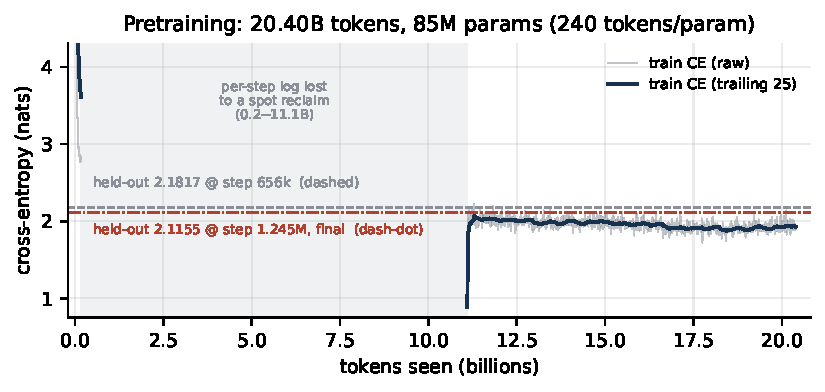
\includegraphics[width=0.99\textwidth]{figs/pretrain.pdf}\\[4pt]
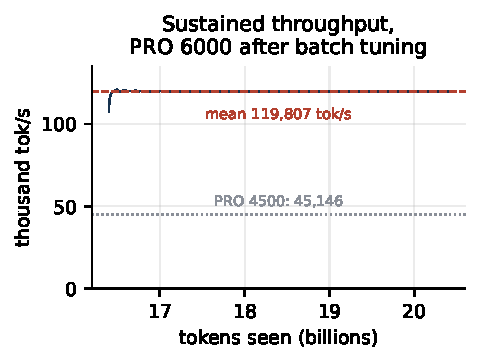
\includegraphics[width=0.49\textwidth]{figs/throughput.pdf}
\hfill
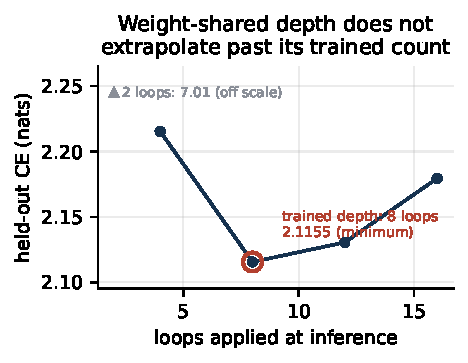
\includegraphics[width=0.49\textwidth]{figs/depth.pdf}
\caption{\textbf{Top:} the pretraining curve, plotted on real token counts from
both metric sources. \emph{The shaded band is a hole in the data, not a
plateau:} the per-step log between $0.10$B and $11.10$B tokens was lost to a
run was interrupted, and the line is broken rather than interpolated --- drawing
through it produced a convincing $11$B-token plateau that never happened. The
single excursion below $1.0$ nat at the right edge of the band is the first
logged step after that resume. The raw series is drawn underneath the trailing
mean deliberately --- see \S\ref{sec:rolling}.
\textbf{Bottom left:} sustained throughput over the final 4.0B tokens.
\textbf{Bottom right:} varying the number of loop applications at inference
time. Held-out loss is minimised at exactly the trained depth ($8$) and rises
at both $4$ and $16$; weight sharing does not buy free depth extrapolation.
The $2$-loop point ($7.01$) is annotated rather than plotted, since clipping it
silently would misrepresent the range.}
\end{figure}

\noindent The model reached $240$ tokens per parameter --- well past
Chinchilla-optimal, and intentionally so, because the downstream stages needed
the strongest possible base at a fixed small size. Three checkpoints were
evaluated on a genuinely held-out split:

\begin{table}[h]
\centering\small
\begin{tabular}{@{}lrrrr@{}}
\toprule
\textbf{Checkpoint} & \textbf{Step} & \textbf{Held-out CE} & \textbf{Code split} & \textbf{Text split} \\
\midrule
baseline & 656{,}711 & 2.1817 & 1.0598 & 3.5910 \\
mid & 910{,}397 & 2.1325 & 1.2693 & 3.4211 \\
\textbf{final} & \textbf{1{,}245{,}117} & \textbf{2.1155} & 1.1979 & 3.3643 \\
\bottomrule
\end{tabular}
\caption{Held-out cross-entropy in nats. The code split improves from baseline
to final but is \emph{worse} at the mid checkpoint --- the corpus mixture
shifted mid-run, and the aggregate number hides that.}
\end{table}

\subsection{Two numerical findings that changed the whole pipeline}

\begin{finding}{BF16 parameters cannot hold optimizer state}
Transformer Engine's NVFP4 path requires BF16 parameters. BF16 spacing near a
value $x$ is $2^{\lfloor \log_2 x \rfloor - 7}$, so any AdamW update smaller
than that rounds away entirely. The consequence was measured, not theorised:
after $657{,}000$ steps, all five RMSNorm gain vectors were still
\emph{bit-exactly} $1.0$, and at the post-training learning rates only $8\%$
(SFT) and $2\%$ (GRPO) of parameter elements could move at all. Without a
fix, SFT was training $8\%$ of the model and GRPO $2\%$.
\emph{Fix:} \code{blackwell\_lm/optim.py} keeps FP32 master weights and copies
back to BF16 after each step, at ${\sim}3\%$ memory overhead.
\end{finding}

\noindent The fix had a trap of its own. Applying masters to \emph{every}
parameter, including the 1-D gains frozen for $657\text{k}$ steps, made the
model \textbf{worse}: held-out loss rose by $0.052$ as stale momentum
discharged into weights that had never moved. The run was rolled back --- both
local weights and the mirrored copy --- to step $656{,}711$, and 1-D gains were left
frozen. A second lesson sits inside the first: an early error in this report's
drafting put that regression at $+0.21$; the difference was drift from an
evaluation set contaminated with early-corpus data, and building a properly
held-out set reduced it to $+0.05$.

\begin{finding}{Flat loss at high learning rate is not saturation}
The training loss was flat for over $1$B tokens and was described --- wrongly ---
as the model having saturated. An anneal probe that dropped the learning rate to
its schedule floor recovered $0.053$ nats in $41$M tokens. The model was
learning-rate-limited, not capacity-limited. ``Saturated'' is a claim about
capacity and requires an anneal probe to support it.
\end{finding}

\section{Supervised fine-tuning}

\begin{figure}[h]
\centering
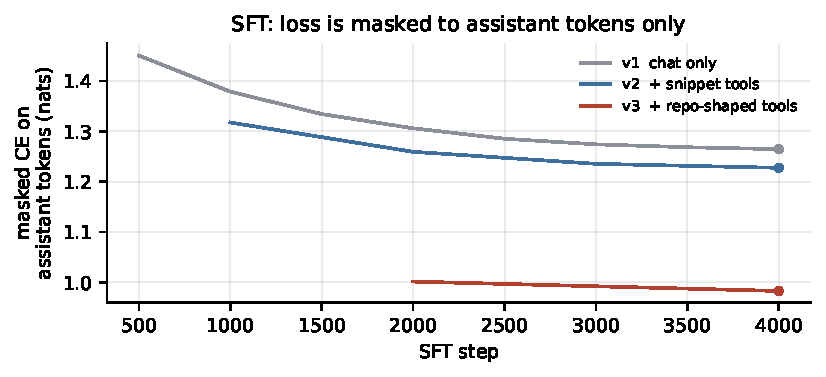
\includegraphics[width=0.72\textwidth]{figs/sft.pdf}
\caption{Masked SFT loss across three data recipes. Loss is computed on
assistant tokens only, via the existing fused cross-entropy kernel's
\code{reduction="none"} path --- no kernel changes were required.}
\end{figure}

\begin{table}[h]
\centering\small
\begin{tabular}{@{}llrrr@{}}
\toprule
\textbf{Run} & \textbf{Data} & \textbf{Masked CE} & \textbf{Format compliance} & \textbf{Tool-call rate} \\
\midrule
v1 & chat only & $2.0056 \rightarrow 1.2648$ & $50\% \rightarrow 100\%$ & $0\% \rightarrow 0\%$ \\
v2 & + synthetic snippet tools & $2.0128 \rightarrow 1.2277$ & $0\% \rightarrow 100\%$ & $0\% \rightarrow 50\%$ \\
\textbf{v3} & + repo-shaped tools & $\mathbf{1.8564 \rightarrow 0.9830}$ & $0\% \rightarrow 100\%$ & $\mathbf{0\% \rightarrow 100\%}$ \\
\bottomrule
\end{tabular}
\caption{Chat-format compliance went from nothing to perfect. The tool-call
rate is the load-bearing column: see \S\ref{sec:convention}.}
\end{table}

\subsection{RL cannot bootstrap a convention the policy never emits}
\label{sec:convention}

The model emitted \code{write\_file} calls with \emph{no} \code{content}
argument $19$ times out of $19$. Three interventions were tried, in order:

\begin{enumerate}
\item \textbf{A more informative error message.} The tool's validator was
changed to return, as data, the exact expected call shape:
\code{write\_file requires 'content'. Expected call: \{"name": ..., "args": ...\}}.
Result: $0/18$. The model could not act on an instruction it could read.
\item \textbf{Reinforcement learning.} With no correct call ever sampled, every
group had identical reward, every group was dropped as zero-variance, and the
policy took $0$ update steps toward the convention.
\item \textbf{Demonstrations.} Repository-shaped SFT trajectories ---
\code{read\_file} $\rightarrow$ \code{write\_file(path, content)} $\rightarrow$
\code{run\_tests} $\rightarrow$ answer, with every tool output produced by real
dispatch rather than written by hand --- took the tool-call rate to $100\%$.
\end{enumerate}

\noindent This pattern recurred three independent times in the project and is
its most portable lesson: \textbf{RL sharpens a distribution, it cannot create
support in it.} If the policy never emits the behaviour, reward shaping has
nothing to reinforce, and the fix is demonstrations.

\section{GRPO with execution-verified rewards}

Rewards come from executing the generated code against hidden tests --- never
from a learned reward model. Sequence-level GSPO ratios, Schulman's $k3$ KL
estimator, DAPO Clip-Higher, and zero-variance group dropping.

\begin{table}[h]
\centering\small
\begin{tabular}{@{}lrrrr@{}}
\toprule
\textbf{Task set} & \textbf{Rollout steps} & \textbf{Update steps} & \textbf{Fully solved} & \textbf{Final mean reward} \\
\midrule
control (12 tasks) & 40 & 76 & 30 & 0.334 \\
MBPP (300 tasks) & 300 & 52 & $9/300$ & 0.0082 \\
\bottomrule
\end{tabular}
\caption{The control set separates a pipeline defect from a capability limit.
The same code that takes $76$ update steps on solvable tasks takes $52$ on
MBPP because $91\%$ of MBPP groups are zero-variance --- the model simply cannot
solve those problems, so there is no gradient. That is a model limit, and the
control run proves it is not a bug.}
\end{table}

\begin{finding}{Two under-powered probes, both corrected}
A tool-call gate measured on $4$ prompts reported rates of exactly $0$, $25$,
$50$, $75$ and $100\%$ --- the only values $4$ samples can produce. Separately,
an SFT A/B at $n{=}60$ showed $+7$pp and was dismissible as noise; re-run at
$n{=}240$ the same comparison gave $+13$pp and was significant. Rate probes in
this report carry standard errors for that reason.
\end{finding}

\section{Agentic reinforcement learning}

Each task becomes a real directory containing a deliberately broken
\code{solution.py}. The agent has four MCP-shaped tools ---
\code{list\_dir}, \code{read\_file}, \code{write\_file}, \code{run\_tests} ---
declared with real JSON Schema, and the system prompt is \emph{generated from
those declarations} so it cannot drift from the dispatcher.

\begin{finding}{The reward reads the file, not the transcript}
An earlier design extracted code from the model's final message. An episode that
ran out of turns mid-tool-call had nothing to extract, scored a flat $0$, made
every group zero-variance, and produced $100$ episodes and $0$ updates. Scoring
the \emph{file the agent leaves behind} is both more faithful to what a coding
agent is for and structurally immune to answer-extraction bugs. The asymmetry is
intended: an agent that edits correctly and says nothing scores full marks, and
one that describes a perfect fix without writing it scores zero.
\end{finding}

\noindent Two further safety properties were adopted after being violated:
scenarios are \textbf{verified breakable} (the reference must pass and the
broken file must fail, in the sandbox, before a scenario is used --- otherwise
an unsolvable task and a broken policy look identical), and \textbf{the harness
owns the grader}. The model was observed inventing its own tests and passing
them; \code{run\_tests(code)} now ignores model-supplied tests entirely.

\begin{figure}[h]
\centering
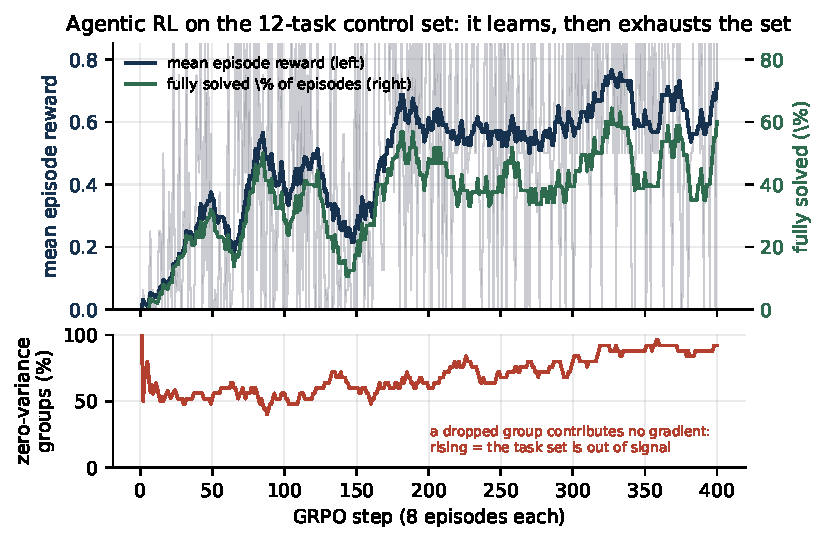
\includegraphics[width=0.76\textwidth]{figs/agent_learning.pdf}
\caption{Agentic RL on the 12-task control set: reward $0.183 \rightarrow 0.656$
and fully-solved $15.6\% \rightarrow 52.5\%$ over $400$ steps ($3{,}200$
episodes, $3{,}413$ update steps). The lower panel is the honest caveat ---
zero-variance groups rise to ${\sim}70\%$ as a 12-task set runs out of signal.}
\end{figure}

\subsection{RL removes any behaviour the reward does not pay for}

Because the reward reads only the final file, calling \code{run\_tests} earned
nothing and cost a turn. The policy responded exactly as instructed.

\begin{figure}[h]
\centering
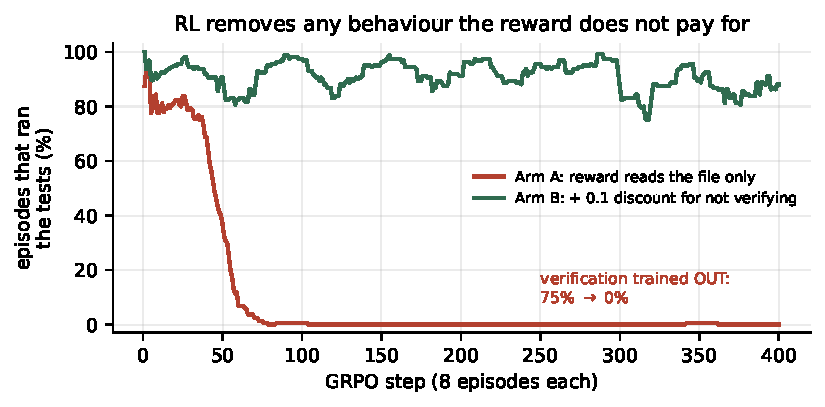
\includegraphics[width=0.76\textwidth]{figs/verify.pdf}
\caption{Arm A pays only for the file. Self-verification is trained
\emph{out}: episodes running the tests fall from $75.3\%$ to $0.0\%$, and tool
errors fall $433 \rightarrow 58$ in lockstep because the errors \emph{were} the
\code{run\_tests} calls. Reward still rose throughout. Arm B adds a $10\%$
discount for finishing unverified and holds verification at $86\%$.}
\end{figure}

\noindent The fix is an incentive, not a patch to the policy. The first
implementation was an additive bonus clamped to $[0,1]$ --- a no-op, since it
can only fire when the reward is already $1.0$ and then clamps straight back.
Worse, the unit test passed it, because the test checked the clamp rather than
checking that the incentive changed any ordering. Reimplemented as a
\emph{discount} for not verifying, with a test asserting the strict ordering
$\text{verified } (1.00) > \text{blind } (0.90) > \text{verified-broken } (0.33)$.

\begin{table}[h]
\centering\small
\begin{tabular}{@{}lrrrr@{}}
\toprule
& \textbf{Arm A} (file-only) & \textbf{Arm B} ($+$verify discount) \\
\midrule
mean episode reward (first $10\%\rightarrow$ last $10\%$) & $0.480 \rightarrow 0.581$ & $0.663 \rightarrow 0.661$ \\
fully solved & $42.5\% \rightarrow 50.9\%$ & $63.4\% \rightarrow 62.5\%$ \\
wrote a file & $79.4\% \rightarrow 80.3\%$ & $91.2\% \rightarrow 86.2\%$ \\
ran the tests & $75.3\% \rightarrow \mathbf{0.0\%}$ & $93.4\% \rightarrow 86.2\%$ \\
own verification passed & --- & $63.7\% \rightarrow 68.4\%$ \\
tool errors (total) & $433$ & $\mathbf{58}$ \\
\bottomrule
\end{tabular}
\caption{$3{,}200$ episodes per arm. Note Arm~B's reward is \textbf{flat}:
$0.663 \rightarrow 0.661$. It began high because its SFT checkpoint was better,
and $400$ steps of RL added nothing --- another instance of demonstrations
outperforming RL at this scale.}
\end{table}

\section{The hardness audit, and the retraction}
\label{sec:hardness}

Arm B's ${\sim}70\%$ solve rate was the project's apparent headline result and
the intended foundation for the next stage. Before building on it, the same
checkpoint was re-probed against \emph{harder breakages of the same tasks}.

\begin{table}[h]
\centering\small
\begin{tabular}{@{}llrrr@{}}
\toprule
\textbf{Tier} & \textbf{How \code{solution.py} is broken} & $n$ & \textbf{Solved} & \textbf{Wrote a file} \\
\midrule
\code{mutate} & one regex substitution ($+ \rightarrow -$) & 120 & $59\% \pm 4$ & $86\% \pm 3$ \\
\code{multi} & two substitutions at once & 120 & $60\% \pm 4$ & $86\% \pm 3$ \\
\code{stub} & function body replaced by \code{pass} & 120 & $\mathbf{0\% \pm 0}$ & $98\% \pm 1$ \\
\code{swap} & a \emph{different} task's real solution & 120 & $\mathbf{0\% \pm 0}$ & $93\% \pm 2$ \\
\bottomrule
\end{tabular}
\caption{\code{stub} and \code{swap} are the honest tiers: neither can be solved
by noticing a suspicious-looking token.}
\end{table}

\begin{retraction}{The 70\% was an artifact. It is withdrawn.}
Zero of $120$ episodes, on two independent honest tiers. The metric was
measuring \emph{``revert the token that looks odd''}, not \emph{``repair the
code''}. A $\mathrm{pass@}12$ follow-up on \code{stub} ($20$ tasks $\times$ $12$
samples $=240$ episodes) found:
\begin{itemize}
\item $\mathrm{pass@}1 = 0.0\%$ \quad ($0/240$ samples)
\item $\mathrm{pass@}12 = 0.0\%$ \quad ($0/20$ tasks \emph{ever} solved)
\item \textbf{any partial credit} $= 0.0\%$ \quad ($0/240$ samples with reward $>0$)
\item final file contents: \textbf{$236$ still the unchanged stub}, $3$ syntax
errors, $1$ valid Python
\end{itemize}
\end{retraction}

\noindent Three things follow, and each is stronger than the last.

\medskip\noindent\textbf{1. The model does not write code; it echoes the file
back.} In $236$ of $240$ episodes the final \code{solution.py} was still the
stub. The agent called \code{read\_file}, then \code{write\_file} with
essentially what it had just read. That is what the $93$--$98\%$ ``wrote a
file'' rate was actually measuring. On the \code{mutate} tier,
copy-with-one-token-changed \emph{is} the correct fix, which is why it scored
$59\%$. Given a stub there is nothing to tweak, so it copies verbatim. The four
exceptions are incoherent: \code{defreduce(a, b):}, \code{defoperations}, and one
sample in which the phrase ``Terms of Service'' bleeds in from pretraining.

\medskip\noindent\textbf{2. Note the direction of the write-rate column.} It is
$93$--$98\%$ on the \emph{hard} tiers --- \emph{higher} than on the easy ones.
The agentic workflow is genuinely learned: the model reads, edits, and verifies,
with $0.07\%$ malformed tool calls. It then writes wrong code with complete
confidence. Tool use and coding are separable capabilities, and at 85M only the
first is reachable.

\medskip\noindent\textbf{3. RL on this tier is structurally impossible, not
merely hard.} Zero partial credit across $240$ samples means every GRPO group
has zero variance and is dropped: \textbf{$0$ update steps, by construction}.
This is the identical failure mode the project already hit once
(\S\ref{sec:convention}), arrived at from the opposite direction.

\subsection{Why this took days to find}
\label{sec:rolling}

The tell was visible from the beginning and was nearly missed: the same
checkpoint solves $9/300$ ($3\%$) of single-turn MBPP while reporting $70\%$ on
repository repair. A $20\times$ gap between \emph{writing} a solution and
\emph{repairing} one should be suspicious on sight. Two habits delayed it:

\begin{itemize}
\item \textbf{A rolling training loss cannot detect any of this.} It missed a
real regression and twice signalled a plateau that was not one. Every quality
claim in this report comes from a fixed held-out set instead --- which is why
Figure~1 plots the raw series underneath the smoothed one.
\item \textbf{A benchmark's difficulty is a parameter, and an unexamined
parameter is an assumption.} The default breakage was a single regex
substitution because that was the easiest thing to implement, and it silently
became the definition of the task.
\end{itemize}

\begin{finding}{What was done about it, in code}
\code{blackwell\_lm/scenario.py} now takes a \code{difficulty} argument
(\code{mutate}/\code{multi}/\code{stub}/\code{swap}), exposed as
\code{--difficulty} on the RL script. A test asserts the property the easy tier
lacked: a stub retains its signature but leaks no \code{return} and no variable
from the original body, a \code{swap} never hands back the reference solution,
and an unknown tier raises rather than silently falling back to the easy one ---
because a refactor that quietly reintroduced a hint would make the benchmark
flattering again, and the number would look like progress.
\end{finding}

\section{The result that only a held-out split could show}
\label{sec:heldout}

Section~\ref{sec:hardness} concluded that the $0/120$ reflected a
code-generation capability limit at 85M. That was traced to a defaulted
argument: \code{train\_sft.py} built every repository demonstration on the
single-token-mutation tier, so the policy had been taught to write a file back
with one token changed, which is exactly what it did ($236/240$ episodes wrote
the unchanged stub back). Rebuilding the demonstrations on the \code{stub} tier
appeared to take $\mathrm{pass@}1$ from $0\%$ to $9.6\%$.

\begin{retraction}{That $9.6\%$ was train accuracy, and so was everything after it}
Training built scenarios from all $374$ MBPP tasks; the scoreboard drew its $20$
from the same pool. Every ``benchmark'' number in this project was therefore
measured on tasks the model had trained on. Nobody had to do anything wrong for
this to happen --- the evaluation harness defaulted to the same task list the
demonstrations were built from, so contamination was the path of least
resistance.
\end{retraction}

\noindent With a real split (300 train, 74 held-out, tasks $901$--$974$) and the
tuned sampling temperature, the same model scores:

\begin{table}[h]
\centering\small
\begin{tabular}{@{}lrr@{}}
\toprule
\textbf{tier} & \textbf{train tasks} & \textbf{HELD-OUT tasks} \\
\midrule
\code{mutate} & $95.0\% \pm 2.0$ & $40.8\% \pm 4.5$ \\
\code{multi}  & $95.0\% \pm 2.0$ & $40.8\% \pm 4.5$ \\
\code{stub}   & $87.5\% \pm 3.0$ & $7.5\% \pm 2.4$ \\
\code{swap}   & $36.7\% \pm 4.4$ & $5.0\% \pm 2.0$ \\
\midrule
mean & $78.5\%$ & $\mathbf{23.5\%}$ \\
\bottomrule
\end{tabular}
\caption{\code{stub} falls from $87.5\%$ to $7.5\%$. The model had memorised
300 reference solutions rather than learned to write function bodies.}
\end{table}

\subsection{The intervention was a net loss, and a contaminated control hid it}

A first comparison used \code{sft\_repo\_heavy}, which scored $73.3\%$ on the
held-out tasks --- but that checkpoint predates the split and had trained on
them. \textbf{A control trained without the same holdout is not a control}, and
it took a second look to notice, because it looked like one.

With a control trained under identical conditions (same 300/74 split,
mutate-only demonstrations), both evaluated on the same 74 unseen tasks at
$T{=}0.2$:

\begin{table}[h]
\centering\small
\begin{tabular}{@{}lrr@{}}
\toprule
\textbf{tier} & \textbf{\code{sft\_ctl}} (mutate only) & \textbf{\code{sft\_ho}} (4 tiers $+$ retry) \\
\midrule
\code{mutate} & $\mathbf{56.7\% \pm 4.5}$ & $40.8\% \pm 4.5$ \\
\code{multi}  & $\mathbf{55.8\% \pm 4.5}$ & $40.8\% \pm 4.5$ \\
\code{stub}   & $0.0\% \pm 0.0$ & $\mathbf{7.5\% \pm 2.4}$ \\
\code{swap}   & $0.0\% \pm 0.0$ & $\mathbf{5.0\% \pm 2.0}$ \\
\midrule
mean & $\mathbf{28.1\%}$ & $23.5\%$ \\
\bottomrule
\end{tabular}
\caption{Training on all four tiers plus retry demonstrations lifts the two
hard tiers off zero and costs ${\sim}16$ points on each easy one: a net
$-4.6$.}
\end{table}

\begin{finding}{At 85M, task-shape priors compete for capacity}
Four of them do not fit. Teaching \code{stub} partly evicts \code{mutate}. The
train-set numbers hid this completely --- there the model held all four tiers
at once ($78.5\%$ mean), because it had \emph{memorised} the solutions, and
memorisation does not trade off the way a learned prior does.
\end{finding}

\section{Sampling temperature was worth more than any training change}

Every agentic number in this project had been measured at $T{=}1.0$, because
that is what the RL rollouts use. $T{=}1.0$ is correct for \emph{exploration} ---
it is what gives GRPO its reward variance --- and wrong for \emph{solving}.
Same checkpoint, no retraining, same 74 held-out tasks, 296 single-turn MBPP
samples:

\begin{table}[h]
\centering\small
\begin{tabular}{@{}lrrr@{}}
\toprule
& $\mathrm{pass@}1$ & $\mathrm{pass@}4$ & emitted a code block \\
\midrule
$T=1.0$ & $1.0\% \pm 0.6$ & $2.7\%$ & $97.6\%$ \\
$T=0.2$ & $\mathbf{6.4\% \pm 1.4}$ & $\mathbf{10.8\%}$ & $100\%$ \\
\bottomrule
\end{tabular}
\caption{$6.4\times$ from one sampling parameter. On the agentic tiers the same
change is worth ${+}24$ points.}
\end{table}

\noindent This settles the \emph{9/300 = 3\%, it cannot write code} headline:
that figure was a $T{=}1.0$ artifact understating the model roughly six-fold. It
is still a weak coder --- $6.4\%$ is not a good score --- but $1\%$ and $6.4\%$
support very different conclusions, and a narrative was built on the former.
The ``still-a-stub'' echo failure also fell from $48/120$ to $11/120$ at
$T{=}0.2$, so part of what was diagnosed as a learned copying prior was a
sampling artifact.

\begin{retraction}{The actual finding of this project}
Four times, an unexamined default produced the result and was credited to the
model:
\begin{enumerate}
\item the \textbf{benchmark tier} --- \code{mutate} made it look capable ($70\%$);
\item the \textbf{training tier} --- \code{mutate} demos made it look incapable ($0/240$);
\item the \textbf{sampling temperature} --- $T{=}1.0$ understated it ${\sim}6\times$;
\item the \textbf{train/test split} --- its absence inflated every number ($78.5\%$ vs $23.5\%$).
\end{enumerate}
Each was chosen because it was the path of least resistance, and each silently
became a definition. Split the tasks and sweep the sampling before believing
anything.
\end{retraction}

\section{Driving a coding CLI with this model}

A working Anthropic-compatible server (\code{serve/anthropic\_shim.py}) serves
the checkpoint, with no Anthropic model anywhere in the loop, so a real client
can drive it via \code{ANTHROPIC\_BASE\_URL}. Two findings.

\medskip\noindent\textbf{The $2{,}048$-token context was not a wall, and
raising it to $32{,}768$ was free.} Measured against a recording server, Claude
Code's first request is ${\sim}18{,}850$ tokens, of which ${\sim}15{,}100$ is
tool JSON Schema. That looked fatal. But \code{max\_seq\_len} never reached the
weights: RoPE is a \emph{non-persistent} buffer rebuilt from config, and with
\code{window=1024} and \code{global\_every\_loop=0} every attention application
is a $1{,}024$-token sliding window, so no relative offset above $1{,}024$ ever
occurs however long the sequence is. Held-out CE on tokens \emph{past} the
$2{,}048$ training length is $1.26$ at $4{,}096$ and $1.16$ at $8{,}192$ ---
no degradation, where broken extrapolation would show CE in the tens. At
$32{,}768$ the server uses $609$\,MiB and answers in $3.6$\,s.

\medskip\noindent\textbf{It connects, and the output is unusable.} With the
whole prompt fitting and $28$k tokens to spare, asked to write and save a
two-number addition function, the model replied with prose about an invented
``\emph{My User GPT}'' and a ``\emph{myapp framework}'': no tool call, no code,
no file. Through the same server with a \emph{short} prompt it writes
\code{def add\_two(a, b): return a + b} correctly. The failure is therefore
prompt distribution, not plumbing and not context: a coding CLI's instruction
blob bears no resemblance to the four-tool, ${\sim}500$-token convention this
policy was trained on. Matching the client's prompt format would be its own
SFT stage.

\section{Reproducibility and artifacts}

All artifacts are mirrored to \code{the project's artifact store}
(13 stage checkpoints and their metrics): 13 stage checkpoints, the tokenizer, per-run metrics as
JSONL, the two audit probes and their logs, and a source tarball. Checkpoint
integrity was verified byte-for-byte against the training host before that host
was terminated.

\begin{finding}{The tokenizer is load-bearing}
A \emph{different} tokenizer silently invalidates every checkpoint --- the
weights load without error and produce nonsense. The exact tokenizer a run used
is published alongside its weights, and its size was verified byte-for-byte
($2{,}290{,}616$ bytes) before teardown.
\end{finding}

\subsection{Operational notes worth carrying forward}

\begin{itemize}
\item \textbf{\code{NVTE\_ALLOW\_UNSAFE\_PICKLE\_EXTRA\_STATE=1}} must be set
before importing Transformer Engine, or every \emph{resume} crashes. Cold starts
look healthy, so this surfaces only when a run is resumed --- the worst possible
moment.
\item \textbf{Build TE with \code{NVTE\_CUDA\_ARCHS=120a}.} The released wheel
silently disables FP4 stochastic rounding on \code{sm\_120}. NVFP4 beat FP8 by
only $8.6\%$ end to end.
\item \textbf{\code{pgrep -f} matches its own command line.} This produced a
process watcher that reported a finished job as still running, indefinitely.
Match on the interpreter and script (\code{pgrep -af "python3 /tmp/x.py"}) and
confirm against GPU memory.
\item \textbf{The sandbox is a robustness boundary, not a containment
boundary.} It applies POSIX rlimits, an isolated interpreter, a throwaway
directory, and process-group kills, but creates no network, mount, or PID
namespace. Run the trainer in a container with no egress if that matters.
\end{itemize}

\section{Conclusions}

\textbf{The pipeline is real and complete.} Pretraining, SFT, GRPO, and
multi-turn agentic RL all ran on real hardware, with FP32 master weights,
MCP-shaped tools, verified scenarios across four difficulty tiers, a
harness-owned grader, and durable metrics. That was the project's stated goal:
prove the pipeline, then point it at a real base model.

\medskip\noindent\textbf{What the model can actually do, on tasks it has never
seen.} It repairs token-level breakage in a real repository $56.7\% \pm 4.5$ of
the time, reading the file, editing it, and verifying with the tests. It writes
a function body from nothing essentially never ($0\%$; $7.5\%$ if trained
specifically for it, at the cost of 16 points on everyday repair). Unaided
single-turn code generation is $6.4\% \pm 1.4$. The agentic \emph{workflow} is
solid --- $90$--$98\%$ write rate, near-zero malformed calls --- and the coding
is weak. Those remain separable, and the workflow is the half that this scale
supports.

\medskip\noindent\textbf{Recommended next steps.} Two, in order.
\emph{(i)} Train on \code{stub}/\code{swap} rather than \code{mutate}
throughout, now that the easy tier is known to flatter in both directions.
$\mathrm{pass@}12 = 40\%$ supplies the variance GRPO needs, so agentic RL on
this tier is now viable at 85M --- it was not before, and the obstacle was the
demonstrations, not the scale. \emph{(ii)} Then run the same stack on an
open-weights coding base in the 7B--30B range with a permissive licence, which
is what the pipeline was built to be pointed at.

\medskip
\begin{center}
\small\color{ink}\itshape
The two results that changed a decision in this project were both negative,
and the second one was a correction of the first.
\end{center}


\end{document}
